% ==================================================================================================================================
% Introduction

L'idée sous-jascente des nombres complexes et d'étendre $\R$ en un corps $\C$ pour être capable de factoriser les polynômes 
irréductibles dans $\R$. On va donc introduire des "nombres" dont le carré sera négatif. 
Pour cela, nous supposerons l'existence d'un $i \in \C$ tel que $i^2 = -1$. 

\minitoc  % Affiche la table des matières pour ce chapitre

% ==================================================================================================================================
% Définition 

\section{Définition et propriétés}

En utilisant le chapitre sur la théorie des corps précédent, on peut définir $\C$ comme une extension de corps de $\R$. 

\begin{definition}[Corps des complexes]
    On définit l'ensemble des nombres complexes, noté $\C$, comme l'extention de corps du corps $\R$ par $i \in \C$ 
    tel que $i$ est racine de $X^2+1 \in \R[X]$. $i$ est donc algébrique sur $\R$ et $i^2 = -1$. 
    On a donc : 
        \[ \C = \R(i) = \R[i] \quad \text{et} \quad [\C : \R] = 2\]
\end{definition}

\subsection{Construction et Opérations}

Commençons tout d'abord par définir formellement l'ensemble des nombres complexes. 

\begin{definition}[Nombres complexes (en tant que quotient)]
    Soit $\R[X]$ l'anneau des polynômes à coefficients réel. On définit l'anneau $\C$ comme le quotient de $\R[X]$ par 
    l'idéal engendré par le polynôme $ X^2+1 \in \R[X]$. On a ainsi : 
        \[ \C := \R[X] / (X^2+1) \] 
    \begin{itemize}
        \item $(X^1 + 1)$ est irréductible dans $\R[X]$ donc $\C$ est un corps. 
        On parlera du \textbf{corps} des complexes. 
        \item Tout élément $z \in \C$ s'écrit de la forme : 
            \[ z = a + Xb, \quad a,b \in \R \] 
        et on identifie $X$ à un élément $ i \in \C$ tel que : 
            \[ i^2 = -1 \] 
    \end{itemize}
    On définit les opérations sur $\C$ de la façon suivante $ \forall a +ib, c+id \in \C$, 
    \begin{itemize}
        \item \textbf{Addition} : 
            \[ (a + ib) + (c + id) = (a+c) + i(b+d) \] 
        \item \textbf{Multiplication} : 
            \[ (a + ib) \times (c + id) = ac + iad + ibc - bd = (ac - bd) + i(ad + bc) \] 
    \end{itemize} 
    On peut donc écrire $\C$ de façon ensembliste comme une extension de $\R$ : 
        \[ \C := \{a + ib \; | \; a,b \in \R\} \] 
\end{definition}

\subsection{Structure de Corps}

\begin{proposition}
    Les propriétés de $\R$ et la construction de $\C$ nous permettent de lui donner une structure de corps. 
    On a donc les propriétés suivantes : 
    \begin{itemize}
        \item L'addition et la multiplication sont associatives et commutatives dans $\C$. 
        \item La multiplication est distributive sur l'addition. 
        \item Il existe des éléments neutres : 
            \[ 1_\C = 1_\R \quad \text{et} \quad 0_\C = 0 + i \times 0 \] 
    \end{itemize}
\end{proposition}

\begin{remark}
    Comme dit en introduction, $\C$ est construit comme extension de $\R$. 
    Ainsi, l'application : 
        \[ \phi : 
            \begin{cases}
                \C \longrightarrow \R \\ 
                a + 0 \times i \longmapsto a 
            \end{cases} \]
    est évidement injective. On peut donc en conlcure que $\R \subset \C$. 
\end{remark}

\begin{proposition}
    $\C$ est un corps de caractéristique nulle. Autrement dit il n'existe pas d'entier $ n \in \N^*$ tel que :
        \[ 1 + \dots + 1 = n \times 1 = 0 \]
\end{proposition}


\begin{theorem}[Théorème Fondamental de l'Algèbre]
    Tout polynômes à coefficients complexes admet au moins une racine dans $\C$. 
    Donc $\C$ est un corps alégriquement clos.
\end{theorem}


% ==================================================================================================================================
% Formes algébrique

\section{Forme algébrique}

Le corps des complexes est assez facile à manipuler étant donné que chacun de ses éléments admets plusieurs formes 
d'écritures (algébrique, exponentielle, trigonométrique) qui permettent d'appréhender des manipulations de différentes 
façons. 

\subsection{Partie Réelle et Imaginaire}

La forme algébrique d'un nombre complexe est sûrement la "plus simple" à comprendre, elle découle directement de 
la définition des nombres complexes comme extension de $\R$. 

\newpage

\begin{definition}[Forme Algébrique d'un nombre complexe]
    Soit $z \in \C$. Alors il existe un unique couple $(a,b) \in \R^2$ tel que : 
        \[ z = a + ib \] 
    On appelle cette forme la \textbf{forme algébrique} de $z$. 
    Ainsi, on définit les parties réelles ($ \Re (z)$) et imaginaires ($ \Im (z)$) de $z$ comme les applications : 
        \[ \Re : 
            \begin{cases}
                \C \longrightarrow \R \\ 
                a + ib \longmapsto a 
            \end{cases}
        \quad \Im : 
            \begin{cases}
                \C \longrightarrow \R \\ 
                a + ib \longmapsto c 
            \end{cases} \] 
    Ce sont deux applications linéaires. 
\end{definition}

\begin{proposition}
    Les parties imaginaires et réelles des nombres complexes nous permettent de les caractériser plus facilement. 
    Ainsi, un nombre complexe est réell ssi sa partie imaginaire est nulle. 
        \[ \text{i.e} \quad z \in \R \iff \Im (z) = 0_\R \] 
\end{proposition}

\begin{remark}
    Grâce à l'unicité des parties réelles et imaginaires, on a les règles d'identification usuelles suivantes : 
        \[ a+ ib = c + id \iff a = c \text{ et } b = d \] 
        \[ a+ ib = 0_\C \iff a = b = 0_\R \] 
\end{remark}

\subsection{Conjugaison}

Dans $\C$ il existe une opération appelée "conjugaison" qui, algébriquement n'a pas trop de signification, mais 
prend tout son sens sous forme trigonométrique. 

\begin{definition}[Conjugaison]
    On définit l'application conjugaison dans les complexes comme : 
    \[ \overline{\bullet} : 
        \begin{cases}
            \C \longrightarrow \C \\ 
            a + i b \longmapsto \overline{a+ib} = a- i b
        \end{cases} \] 
    On appelera $\overline{z}$ le conjugué de $z$ dans $\C$. 
\end{definition}

\begin{prop}[Conjugaison]
    \begin{itemize}
        \item La conjugaison est \textbf{involutive}. 
            \[ \text{i.e} \quad \forall z \in \C, \overline{\overline{z}} = z \] 
        \item La conjugaison est \textbf{linéaire}. 
        \item La conjugaison respecte la multiplication. 
            \[ \text{i.e} \quad \forall z,z' \in \C, \overline{z . z'} = \overline{z} \times \overline{z'} \]
        \item Pour tout $z \in \C$ on a les propriétés suivantes : 
            \[ \Re(z) = \frac{z + \overline{z}}{2} \quad \text{et} \quad \Im(z) = \frac{z - \overline{z}}{2i} \] 
    \end{itemize}
\end{prop}

\subsection{Module d'un nombre complexe}

Tout comme la conjugaison, le module d'un nombre complexe n'a pas beaucoup de signification sous forme algébrique 
mais il peut s'interpréter comme une norme dans $\C$. 

\begin{definition}[Module d'un nombre complexe]
    On appelle module dans $\C$ l'application : 
        \[ | \cdot | : 
            \begin{cases}
                \C \longrightarrow \R_+ \\ 
                z = a + ib \longmapsto \sqrt{z \overline{z}} = \sqrt{a^2 + b^2}
            \end{cases} \] 
    On appelera ainsi module de $z$ dans $\C$ le réel positif $\sqrt{z \overline{z}}$. 
\end{definition}

Tout comme la conjugaison, le module possède quelque propriétés bien utiles. 

\begin{prop}[Module]
    \begin{itemize}
        \item Le module est défini. 
            \[ \text{i.e} \quad \forall z \in \C, \quad | z | = 0_\R \iff z = 0_\C \] 
        \item Le module est positif ($ \forall z \in \C, |z| \geqslant 0$). 
        \item Le module respecte la multiplication. 
            \[ \text{i.e} \quad \forall z, z' \in \C, \quad | z \times z'| = |z| \times |z'| \] 
        \item Le module vérifie l'inégalité triangulaire :
            \[ \forall z, z' \in \C, \quad | z + z' | \leqslant | z | + |z '| \] 
    \end{itemize}
\end{prop}

\begin{remark}
    On peut remarque que le module vérifie toutes les conditions pour être une norme. 
    En effet, \textbf{le module est une norme sur $\C$}. 
    De plus, il est bien compatible avec la norme réelle (valeur absolue) puisque : 
        \[ \forall a \in \R, \quad \sqrt{a \times \overline{a}} = \sqrt{a^2} = |a| \] 
\end{remark}

% ==================================================================================================================================
% Forme Trigonométrioque d'un nombre complexe 

\section{Forme Trigonométrique d'un nombre complexe}

La forme trigonométrique d'un nombre complexe est moins facilement manipulable algébriquement mais reste très utile. 
En effet, elle permet de représenter facilement n'importe quel nombre complexe dans le plan. 

\begin{definition}[Forme Trigonométrique]
    Soit $z = a + ib \in \C$. On définit la forme trigonométrique de $z$ comme : 
        \[ z = r (\cos \theta + i \sin \theta) \] 
    où : 

    \begin{minipage}{0.45\textwidth}
        \begin{itemize}
            \item $ r = | z | = \sqrt{a^2 + b^2} $ 
            \item $\theta$ est appelé \textbf{argument de }$z$. Il représente l'angle que fait $z$ 
            avec l'axe des réels dans le plan. 
        \end{itemize}
    \end{minipage}
    \hfill
    \begin{minipage}{0.45\textwidth}
        \begin{center}
            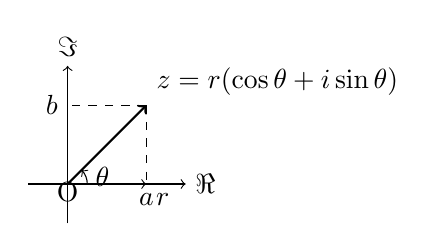
\begin{tikzpicture}[scale=0.5]
                % Dessin des axes
                \draw[->] (-1,0) -- (3,0) node[right] {$\Re$};  % axe réel
                \draw[->] (0,-1) -- (0,3) node[above] {$\Im$};  % axe imaginaire
            
                % Représentation du nombre complexe
                \draw[->,thick] (0,0) -- (2,2) node[above right] {$z = r(\cos \theta + i \sin \theta)$};
            
                % Dessin de l'angle
                \draw[->] (0.5,0) arc[start angle=0, end angle=45, radius=0.5] node[midway, right] {$\theta$};
            
                % Représentation du module r
                \draw[dashed] (2,2) -- (2,0) node[below] {$a$};
                \draw[dashed] (2,2) -- (0,2) node[left] {$b$};
                \draw[->] (0,0) -- (2,0) node[below right] {$r$};
                
                % Point d'origine
                \node at (0,-0.2) {O};
            \end{tikzpicture}
        \end{center}
    \end{minipage}
\end{definition}

\subsection{Nombres complexes de module 1}

On peur remarquer, parmi les nombres complexes que ceux de moldule $1$ sont assez caractéristiques. 
On note l'ensemble des nombres complexes de module 1 $\U$ défini par : 
    \[ \U := \{z \in \C,  \; | z | = 1 \} \] 
Les nombres complexes forment ainsi ce que l'on appelle le \textbf{cercle trigonométrique} dans le plan : 

\begin{center}
    \resizebox{0.7\textwidth}{!}{
    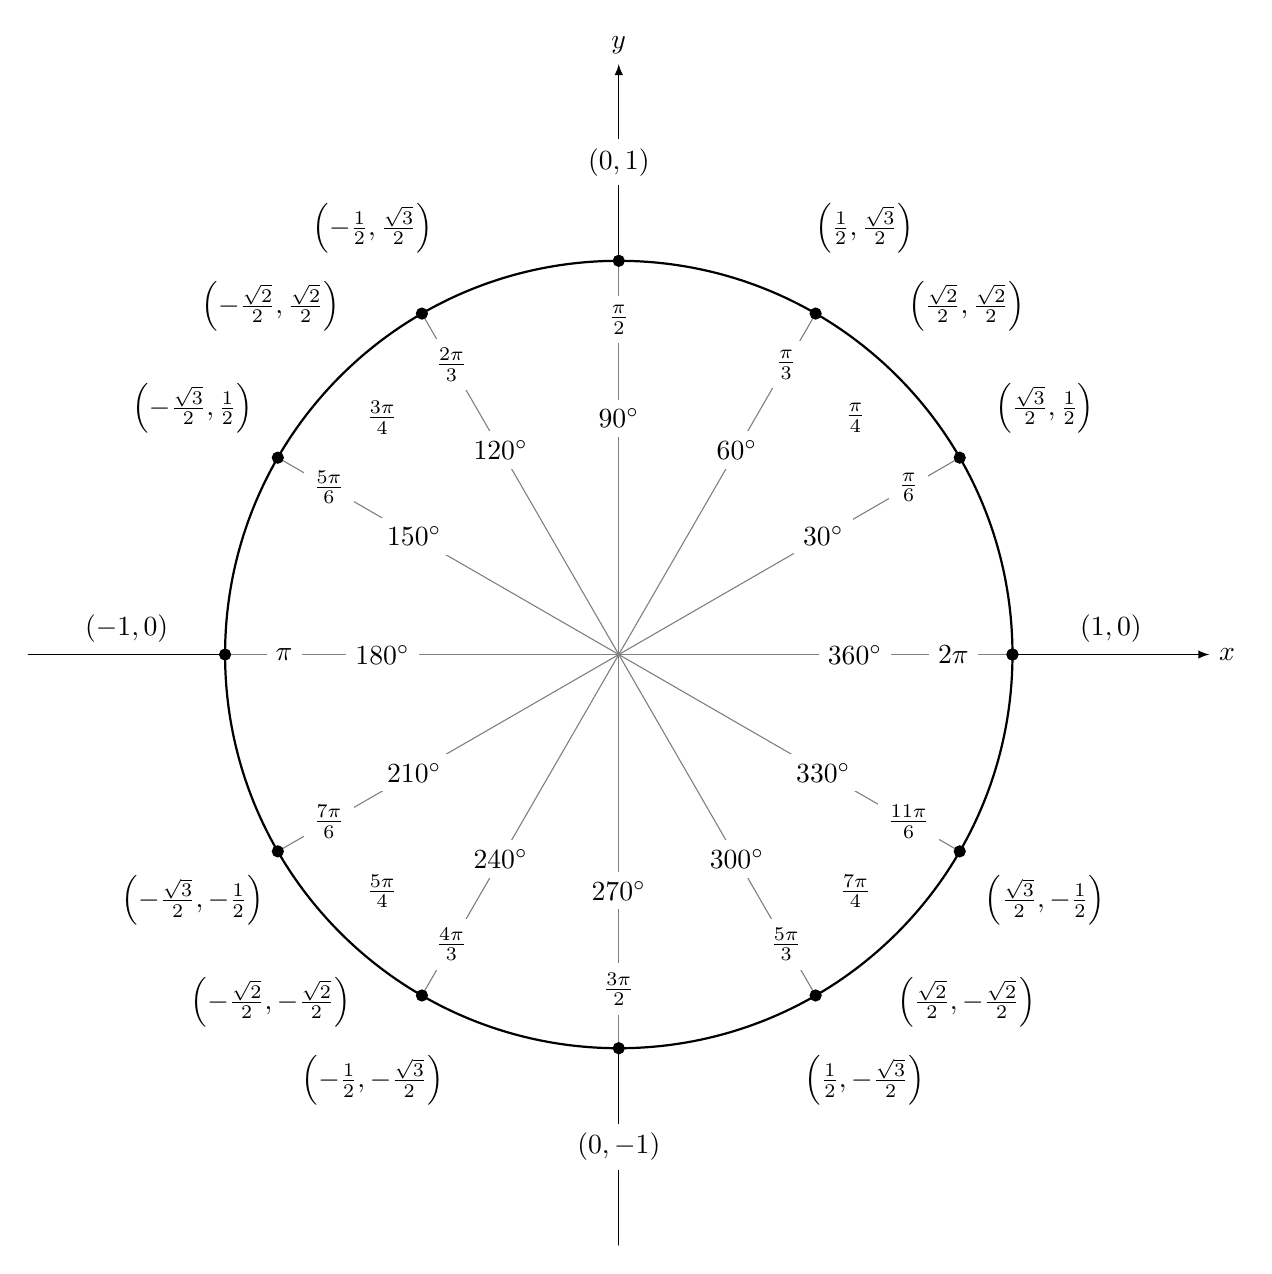
\begin{tikzpicture}[scale=5,cap=round,>=latex]
        % draw the coordinates
        \draw[->] (-1.5cm,0cm) -- (1.5cm,0cm) node[right,fill=white] {$x$};
        \draw[->] (0cm,-1.5cm) -- (0cm,1.5cm) node[above,fill=white] {$y$};

        % draw the unit circle
        \draw[thick] (0cm,0cm) circle(1cm);

        \foreach \x in {0,30,...,360} {
                % lines from center to point
                \draw[gray] (0cm,0cm) -- (\x:1cm);
                % dots at each point
                \filldraw[black] (\x:1cm) circle(0.4pt);
                % draw each angle in degrees
                \draw (\x:0.6cm) node[fill=white] {$\x^\circ$};
        }

        % draw each angle in radians
        \foreach \x/\xtext in {
            30/\frac{\pi}{6},
            45/\frac{\pi}{4},
            60/\frac{\pi}{3},
            90/\frac{\pi}{2},
            120/\frac{2\pi}{3},
            135/\frac{3\pi}{4},
            150/\frac{5\pi}{6},
            180/\pi,
            210/\frac{7\pi}{6},
            225/\frac{5\pi}{4},
            240/\frac{4\pi}{3},
            270/\frac{3\pi}{2},
            300/\frac{5\pi}{3},
            315/\frac{7\pi}{4},
            330/\frac{11\pi}{6},
            360/2\pi}
                \draw (\x:0.85cm) node[fill=white] {$\xtext$};

        \foreach \x/\xtext/\y in {
            % the coordinates for the first quadrant
            30/\frac{\sqrt{3}}{2}/\frac{1}{2},
            45/\frac{\sqrt{2}}{2}/\frac{\sqrt{2}}{2},
            60/\frac{1}{2}/\frac{\sqrt{3}}{2},
            % the coordinates for the second quadrant
            150/-\frac{\sqrt{3}}{2}/\frac{1}{2},
            135/-\frac{\sqrt{2}}{2}/\frac{\sqrt{2}}{2},
            120/-\frac{1}{2}/\frac{\sqrt{3}}{2},
            % the coordinates for the third quadrant
            210/-\frac{\sqrt{3}}{2}/-\frac{1}{2},
            225/-\frac{\sqrt{2}}{2}/-\frac{\sqrt{2}}{2},
            240/-\frac{1}{2}/-\frac{\sqrt{3}}{2},
            % the coordinates for the fourth quadrant
            330/\frac{\sqrt{3}}{2}/-\frac{1}{2},
            315/\frac{\sqrt{2}}{2}/-\frac{\sqrt{2}}{2},
            300/\frac{1}{2}/-\frac{\sqrt{3}}{2}}
                \draw (\x:1.25cm) node[fill=white] {$\left(\xtext,\y\right)$};

        % draw the horizontal and vertical coordinates
        % the placement is better this way
        \draw (-1.25cm,0cm) node[above=1pt] {$(-1,0)$}
              (1.25cm,0cm)  node[above=1pt] {$(1,0)$}
              (0cm,-1.25cm) node[fill=white] {$(0,-1)$}
              (0cm,1.25cm)  node[fill=white] {$(0,1)$};
    \end{tikzpicture}}
\end{center}

\begin{remark}
    On peut aussi remarquer que l'inverse d'un nombre complexe de module 1 est exactement son conjugué. 
\end{remark}


% ==================================================================================================================================
% Forme exponentielle

\section{Forme Exponentielle d'un nombre complexe}

Enfin, nous pouvons définir la forme exponentielle d'un nombre complexe. 

\begin{definition}[Forme Exponentielle]
    Soit $z = r (\cos \theta + i \sin \theta) \in \C^*$. On définit sa forme exponentielle ou polaire comme : 
        \[ z = r e^{i \theta} \] 
\end{definition}

\begin{remark}
    La forme exponentielle d'un nombre complexe est unique modulo $2 \pi$ pour $ \theta$. 
    \[ \text{i.e} \quad \forall r_1 e^{i\theta_1},  r_2 e^{i \theta_2} \in \C, \quad r_1 e^{i\theta_1} = r_2 e^{i \theta_2} \iff 
    \begin{cases}
        r_1 = r_2 \\ 
        \theta_1 \underset{2\pi}{\equiv } \theta_2 
    \end{cases} \] 
\end{remark}

\begin{prop}[Formule de Moivre]
    Soit $\theta \in \R$ et $ n \in \Z$ on a alors la formule suivante, dite de Moivre : 
        \[ \left(e^{i\theta} \right)^n = e^{ni\theta} \] 
    en notation troginométrique, on a donc : 
        \[ \left( \cos \theta + i \sin \theta \right)^n = \cos n\theta + i \sin n \theta \] 
\end{prop}

\begin{proposition}[Exponentielle complexe de module 1]
    Pour les exponentielles complexes de module 1, on a différentes propriétés notamment les formules d'Euler : 
        \[ \forall \theta \in \R, \quad \cos \theta = \frac{e^{i\theta} + e^{-i\theta}}{2} \; \text{et} \; \sin \theta = \frac{e^{i\theta} - e^{-i\theta}}{2i} \] 
    Mais aussi :
    \begin{itemize}
        \item $ \forall z \in \C, \quad |z| = 1 \iff \exists \theta \in \R, z = e^{i\theta} $ 
        \item $ \forall \theta \in \R, \quad \overline{e^{i\theta}} = e^{i-\theta} $ 
        \item $ \forall p,q \in \R, \quad e^{i (p+q)} = e^{ip} \times e^{iq} $ 
    \end{itemize} 
\end{proposition}














